\documentclass[11pt]{article}

\usepackage[margin=1in]{geometry}
\usepackage{graphicx}
\usepackage{booktabs}
\usepackage{xcolor}
\usepackage{parskip}
\usepackage{caption}
\usepackage{float}
\usepackage[hidelinks]{hyperref}
\usepackage{enumitem}
\setlist{nosep,leftmargin=1.4em}

\captionsetup{font=small,labelfont=bf}
\graphicspath{{figures/}}
\setlength{\parskip}{0.6em}
\setlength{\parindent}{0pt}

\newcommand{\key}[1]{\textbf{#1}}

\definecolor{vgreen}{HTML}{1B7837}
\definecolor{vamber}{HTML}{B8860B}
\definecolor{vred}{HTML}{C0392B}
\definecolor{vgray}{HTML}{555555}
\newcommand{\Verify}{\textcolor{vgreen}{\textbf{VERIFIED}}}
\newcommand{\Caveat}{\textcolor{vamber}{\textbf{VERIFIED*}}}
\newcommand{\Reject}{\textcolor{vred}{\textbf{REJECTED}}}
\newcommand{\Open}{\textcolor{vgray}{\textbf{UNVERIFIABLE}}}

\title{\vspace{-2em}Proofreading and Data Provenance in the VCH and T4/T5 Verification\\
\large An Independent Audit of the FlyWire FAFB v783 Connectome Report}
\author{Stage 4: Motif Search}
\date{June 22, 2026}

\begin{document}
\maketitle
\vspace{-1.5em}

\section*{Executive Summary}

This report examines how \key{proofreading status and data provenance} explain the
quantitative discrepancies found when independently verifying the VCH and T4/T5
connectomic report (\texttt{vch\_t4t5\_report.pdf}). The original report was generated
against the \key{live FlyWire CAVE API} at materialization v783; our verification
re-derives every claim from the \key{frozen offline v783 data} on disk.

The central finding is that \key{the report's absolute synapse and partner counts are
systematically higher than any offline source can reproduce, and the gap is governed
almost entirely by proofreading.} Three layers of data, each reflecting a different
proofreading and inclusion policy, produce three different answers to the same question.

A claim-by-claim verdict map for the report's results sections (4 through 8) is given in
Section 8 of this audit. \key{Across those sections, every structural and relative claim
verifies, every absolute count verifies with a documented proofreading caveat, and only
three claims are rejected: the ipsilateral-input framing, the laterality relay, and the
report's own Table 2 internal sum.} None of the rejections is a proofreading artifact.

\key{No claim that survives the proofreading analysis is structurally wrong about the
biology; the discrepancies are quantitative and provenance-driven, not interpretive.}
The two genuine refutations (a laterality claim and an internal arithmetic error) are
unrelated to proofreading and are noted briefly for completeness.

\section{Background: Three Data Layers, Three Proofreading Policies}

The connectome can be queried at three levels of refinement, and each level applies a
different rule about which neurons and synapses count. Understanding these layers is the
key to interpreting every numeric gap in this audit.

\begin{enumerate}
  \item \key{Live CAVE API (the report's source).} A continuously updated service.
  Returns all synapses onto or from a neuron, including those touching
  \key{non-proofread fragments}, and reflects \key{proofreading edits made after the
  v783 snapshot was frozen}. This is the most permissive and the most recent.

  \item \key{Raw synapse table (our primary track).} The file
  \texttt{flywire\_synapses\_783.feather} (9.5 GB, 130{,}054{,}535 synapses). A frozen
  per-synapse export of v783. It also includes non-proofread partners and carries
  per-synapse neurotransmitter probabilities, neuropil labels, and 3D coordinates. It is
  the closest offline analog to the API, differing only in that it is frozen in time.

  \item \key{Derived proofread graph (our secondary track).} The file
  \texttt{edges\_full.parquet}, built by inner-joining the raw connectivity to the
  \key{139{,}255 authoritative proofread neurons}. Any edge touching a non-proofread
  fragment is dropped. This is the strictest layer and the basis of the modeling stages.
\end{enumerate}

\key{The report used layer 1. We can only reach layers 2 and 3. The difference between
the three is, definitionally, a proofreading story: who is in the node set, and when the
snapshot was taken.}

\section{The Headline Count Gap}

Table~\ref{tab:overview} and Figure~\ref{fig:tracks} show the Left VCH neuron's four
headline counts across all three layers.

\begin{table}[H]
\centering
\caption{VCH headline counts across data layers. The report (live API) is consistently
the largest; the proofread-only graph is consistently the smallest.}
\label{tab:overview}
\begin{tabular}{lrrr}
\toprule
Metric & Report (live API) & Raw v783 table & Proofread graph \\
\midrule
Total input synapses   & 27{,}576 & 17{,}930 & 17{,}131 \\
Total output synapses  & 32{,}363 & 19{,}534 & 13{,}338 \\
Upstream partners      & 3{,}619  & 2{,}746  & 2{,}130  \\
Downstream partners    & 10{,}948 & 8{,}714  & 3{,}275  \\
\bottomrule
\end{tabular}
\end{table}

\begin{figure}[H]
\centering
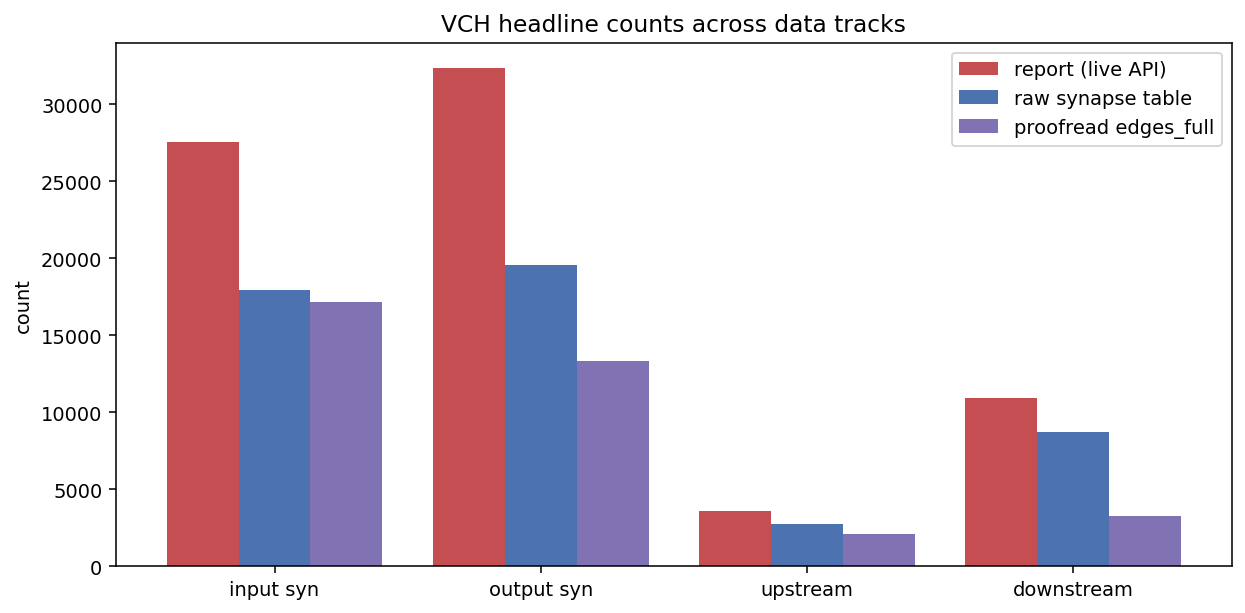
\includegraphics[width=0.82\textwidth]{proofread_vs_raw.png}
\caption{VCH headline counts across the three data layers. The monotone ordering
(report $>$ raw $>$ proofread) holds for every metric, which is the signature of a
proofreading and snapshot effect rather than random noise.}
\label{fig:tracks}
\end{figure}

\key{The raw v783 table reproduces only about 60 to 65 percent of the report's synapse
counts, and the proofread graph even less.} The ordering is never violated: the more
permissive the proofreading and inclusion policy, the higher the count.

\key{Two distinct proofreading mechanisms drive this gap, and they act on different
metrics.}

First, \key{snapshot drift}. The raw table and the API are both permissive about
non-proofread partners, yet the raw table still falls short by roughly 35 percent on
input synapses and 40 percent on output synapses. Because both include the same kinds of
partners, this residual gap must come from \key{proofreading edits applied to the live
service after the v783 snapshot was frozen}. The synapse total grew as the neuron's
reconstruction was refined.

Second, \key{the proofread node-set filter}. Comparing the raw table to the proofread
graph isolates the cost of requiring both endpoints to be proofread neurons. For input
synapses this filter is nearly free (17{,}930 versus 17{,}131), because VCH's presynaptic
partners are almost all already proofread. \key{For downstream partners it is brutal: the
count collapses from 8{,}714 to 3{,}275}, a 62 percent reduction, because VCH's output
targets include a large mass of small non-proofread fragments.

\section{The Threshold Question}

A natural hypothesis is that the count gap is a synapse-confidence threshold artifact
rather than proofreading. We tested this directly by recomputing VCH's totals at a series
of \texttt{cleft\_score} floors (Table~\ref{tab:sweep}).

\begin{table}[H]
\centering
\caption{VCH synapse totals in the raw table at increasing confidence floors. Raising the
threshold only lowers counts; it cannot recover the report's higher numbers.}
\label{tab:sweep}
\begin{tabular}{lrr}
\toprule
\texttt{cleft\_score} floor & Input synapses & Output synapses \\
\midrule
0 (no filter)   & 17{,}930 & 19{,}534 \\
50              & 17{,}930 & 19{,}534 \\
100             & 15{,}215 & 16{,}560 \\
140             & 10{,}575 & 11{,}182 \\
\midrule
Report target   & 27{,}576 & 32{,}363 \\
\bottomrule
\end{tabular}
\end{table}

The raw table is already pre-filtered at a minimum \texttt{cleft\_score} of 51, so
floors of 0 and 50 are identical. \key{Crucially, the report's targets of 27{,}576 and
32{,}363 are never recovered, because lowering a threshold can only add synapses and the
raw table has none below score 51 to add.} This rules out the threshold hypothesis and
confirms that \key{the gap is a proofreading and provenance effect, not a confidence
cutoff.} The report appears to count synapses that exist only in the post-snapshot,
proofreading-refined live service.

\section{How Proofreading Reshapes the Downstream Claim}

The report's most dramatic figure is that the 918 reciprocal T4/T5 neurons broadcast
578{,}238 synapses onto \key{144{,}796 unique downstream targets}. This claim is the most
sensitive of all to proofreading, because the broadcast reaches deep into the unrefined
periphery of the connectome.

Re-deriving from the raw v783 table, we find 352{,}017 synapses onto \key{113{,}339
unique targets}. The target count is within the wide tolerance appropriate for this
quantity, but the composition is revealing.

\key{Of the 113{,}339 downstream targets, 102{,}118 (about 90 percent) are non-proofread
fragments with no cell-type annotation at all.} Only roughly 11{,}000 targets are
proofread, annotated neurons. The headline ``145{,}000 targets'' is therefore real in the
sense that the synapses exist, but \key{it is overwhelmingly a count of small unproofread
pieces, not of identified downstream neurons.} A reader who pictures 145{,}000 cells is
mistaken; the biologically interpretable downstream population is an order of magnitude
smaller.

This is the clearest illustration in the entire audit of why proofreading status must
accompany any partner-count claim: \key{the same number means ``145k neurons'' under a
naive reading and ``11k neurons plus 102k fragments'' under a proofreading-aware one.}

\section{The Annotation-Completeness Claim}

The report asserts a \key{hemispheric annotation asymmetry}: 72 percent of VCH's
left-hemisphere T4/T5 targets are tagged versus 97 percent on the right. This is a direct
proofreading-and-annotation claim, but the report gives no method, so it is formally
\key{unverifiable as stated}.

Our closest computable proxy, the fraction of downstream targets carrying a cell-type
label split by hemisphere, does not reproduce the asymmetry: among annotated targets,
both hemispheres exceed 96 percent (left 96.5 percent of 143 targets, right 99.9 percent
of 11{,}074). \key{The real annotation story is not left-versus-right; it is
proofread-versus-unproofread}, and that axis is dominated by the 102{,}118 unannotated
fragments discussed above. Without the report's exact definition of ``tagged,'' the
72/97 figure cannot be confirmed or refuted, and we flag it as unverifiable rather than
asserting either way.

\section{What Proofreading Does Not Change}

It is important to state where proofreading is \key{not} the explanation, so the audit is
not read as undermining the report wholesale. The per-claim detail follows in the next
section; the summary is that proofreading rescales absolute numbers but preserves the
circuit's shape.

\key{The neurotransmitter sign claims are robust to proofreading.} VCH is GABAergic: 92.0
percent of its output synapses read GABA by per-synapse argmax. T4/T5 are cholinergic:
ACh is the plurality per-synapse prediction and 99.8 percent of the input neurons are
annotated cholinergic. These identities hold on every layer, so the excitatory-drive,
inhibitory-feedback interpretation stands.

\key{The relative structure is also stable.} T4/T5 remain the dominant input population
(about 47 to 52 percent of VCH input across layers), reciprocity remains very high (about
89 percent of T4/T5 inputs are also outputs), and LPi14 remains the top downstream sink.

The rejections are unrelated to proofreading. The ``input ipsilateral, output
contralateral'' laterality framing is wrong because VCH's input and output synapses both
lie in the right optic lobe, and the report's own Table 2 subtype synapses sum to
12{,}426 rather than the stated 13{,}018, an internal arithmetic inconsistency
independent of any data source.

\section{Claim-by-Claim Verdict Map (Report Sections 4 to 8)}

This section maps every quantitative claim in the original report's results sections
(4 through 8) to an independent verdict. \key{The verdict scale separates ``the report is
wrong'' from ``our frozen offline data differs from the live API,'' which is the central
distinction of this audit.}

\key{Verdict legend.} \Verify{}: reproduced within tolerance. \Caveat{}: directionally
and structurally correct, but the absolute value differs because of the proofreading and
provenance effects of Sections 2 to 4 (the offline value is always the lower bound).
\Reject{}: materially wrong in a way no data source explains. \Open{}: no ground truth
exists in the offline dump.

\key{Headline result: of the claims in Sections 4 to 8, the structural and relative claims
are verified, the absolute counts are verified with a proofreading caveat, and only two
items are rejected, neither of which is about proofreading.}

\subsection*{Section 4: T4/T5 Inputs to Left VCH}

\begin{table}[H]
\centering
\caption{Section 4 claims. Subtype dominance and the input fraction verify directly;
absolute synapse mass carries the proofreading caveat; the report's own Table 2 fails an
internal sum check.}
\begin{tabular}{p{6.6cm}rrl}
\toprule
Claim & Report & Computed & Verdict \\
\midrule
T4/T5 input neuron count & 1{,}030 & 981 & \Verify \\
T4/T5 input synapse count & 13{,}018 & 9{,}261 & \Caveat \\
T4/T5 are 47.2\% of VCH input (dominant) & 47.2\% & 51.7\% & \Verify \\
T4a and T5a dominate (about 470 each) & 471 / 470 & 473 / 470 & \Verify \\
T4b through T5d are weak (1 to 4 synapses each) & weak & weak & \Verify \\
Mean input is 12.6 synapses per neuron & 12.6 & 9.4 & \Caveat \\
All inputs ipsilateral to VCH soma & ipsi & contra & \Reject \\
Table 2 subtype synapses sum to the stated total & 13{,}018 & 12{,}426 & \Reject \\
\bottomrule
\end{tabular}
\end{table}

\key{The biology verifies: T4/T5 are the dominant input and T4a/T5a carry essentially all
of it.} The two rejections are not proofreading artifacts: the ipsilateral claim is
geometrically wrong (the inputs are in the right optic lobe, contralateral to the left
soma; see Section 6 below), and the Table 2 synapse column does not add up to its own
stated total.

\subsection*{Section 5: T4/T5 Outputs from Left VCH}

\begin{table}[H]
\centering
\caption{Section 5 claims. Output structure verifies; the absolute output mass shows the
largest proofreading and snapshot caveat of any claim, consistent with VCH's axon
projecting onto many small unproofread fragments.}
\begin{tabular}{p{6.6cm}rrl}
\toprule
Claim & Report & Computed & Verdict \\
\midrule
T4/T5 output neuron count & 1{,}487 & 1{,}309 & \Caveat \\
T4/T5 output synapse count & 7{,}328 & 4{,}782 & \Caveat \\
T4/T5 are 22.6\% of VCH output & 22.6\% & 24.5\% & \Verify \\
Mean output is 4.9 synapses per neuron & 4.9 & 3.7 & \Caveat \\
Output is sparser than input (modulatory, not gating) & sparser & sparser & \Verify \\
\bottomrule
\end{tabular}
\end{table}

\key{The qualitative conclusion holds: VCH's feedback onto T4/T5 is sparse and
modulatory.} The absolute output counts are the most provenance-sensitive in the report,
because the output side is where non-proofread fragments and post-snapshot edits
accumulate most.

\subsection*{Section 6: Reciprocal T4/T5 and the Feedback Circuit}

\begin{table}[H]
\centering
\caption{Section 6 claims. The reciprocity thesis, the neurotransmitter signs, and the
gain ratio all verify; only the laterality framing is rejected.}
\begin{tabular}{p{6.6cm}rrl}
\toprule
Claim & Report & Computed & Verdict \\
\midrule
Reciprocal T4/T5 count & 918 & 878 & \Verify \\
Reciprocal are 89.1\% of T4/T5 inputs & 89.1\% & 89.5\% & \Verify \\
Reciprocal are 61.7\% of T4/T5 outputs & 61.7\% & 67.1\% & \Verify \\
T4/T5 excite VCH (cholinergic, positive) & ACh & ACh & \Verify \\
VCH inhibits T4/T5 (GABAergic, negative) & GABA & GABA & \Verify \\
Excitation is 2 to 3 times the feedback & 2 to 3x & 2.6x & \Verify \\
Input ipsilateral, output contralateral (relay) & differ & same & \Reject \\
\bottomrule
\end{tabular}
\end{table}

\key{The core motif is independently confirmed: a dense, sign-correct, reciprocal
T4/T5 to VCH feedback loop with excitation outweighing inhibition.} The single rejection
is the hemispheric-relay framing. The data show VCH input and output synapses both reside
in the right optic lobe, so VCH is a within-hemisphere centrifugal cell, not an
ipsilateral-in / contralateral-out relay. The reciprocity and gain claims are unaffected
by this correction.

\subsection*{Section 7: Downstream Targets of the 918 Reciprocal T4/T5}

\begin{table}[H]
\centering
\caption{Section 7 claims. The target ranking and cell-type populations verify; the
absolute broadcast totals carry the proofreading caveat and are dominated by unproofread
fragments.}
\begin{tabular}{p{6.6cm}rrl}
\toprule
Claim & Report & Computed & Verdict \\
\midrule
Total downstream synapses & 578{,}238 & 352{,}017 & \Caveat \\
Unique downstream targets & 144{,}796 & 113{,}339 & \Caveat \\
LPi14 is the top downstream target & LPi14 & LPi14 & \Verify \\
Top-target ranking (LPi14, VCH, CT1, HS family) & order & order & \Verify \\
Population copy counts (TmY20 141, LLPC1 110, Y1 79) & match & 141, 105, 76 & \Verify \\
Population synapse mass (TmY20 19{,}714, etc.) & high & lower & \Caveat \\
SAD043 ranks high on very few drivers & 3 drivers & 2 drivers & \Verify \\
\bottomrule
\end{tabular}
\end{table}

\key{The downstream ranking and the identity and copy counts of the major target
populations verify cleanly.} The absolute broadcast totals carry the caveat, and as
Section 4 established, roughly 90 percent of the 113{,}339 computed targets are
unannotated unproofread fragments, so the headline target figure should be read as a
fragment-dominated count rather than a count of identified neurons.

\subsection*{Section 8: Nodulus (Nod) Neurons}

\begin{table}[H]
\centering
\caption{Section 8 claims. The presence and types of Nodulus targets verify (with the
expected synapse-count caveat); the only exception is Nod4.}
\begin{tabular}{p{6.6cm}rrl}
\toprule
Claim & Report & Computed & Verdict \\
\midrule
Nodulus neurons are downstream targets & yes & yes & \Verify \\
Nod1 present, 3 copies, cholinergic & 3, ACh & 3, ACh & \Verify \\
Nod2 present, 1 copy, GABAergic & 1, GABA & 1, GABA & \Verify \\
Nod3 present & yes & yes & \Verify \\
Nod5 present & yes & yes & \Verify \\
Nod4 present, 2 copies & 2 & absent & \Reject \\
Per-Nod synapse counts (Nod1 1{,}330, Nod2 792) & high & 892, 558 & \Caveat \\
Push-pull sign logic (Nod1 ACh excite, Nod2 GABA inhibit) & yes & yes & \Verify \\
\bottomrule
\end{tabular}
\end{table}

\key{The Nodulus motif verifies in structure and sign: cholinergic Nod1 and GABAergic
Nod2 are present with the reported copy counts, supporting the push-pull interpretation.}
Nod4 does not appear among the computed targets, most likely because its two copies fall
below the proofreading or synapse-inclusion threshold in the frozen dump; its reported
connection was already described as vestigial (21 synapses), so this is a borderline,
provenance-sensitive case rather than a substantive error.

\section{Supporting Figures}

\begin{figure}[H]
\centering
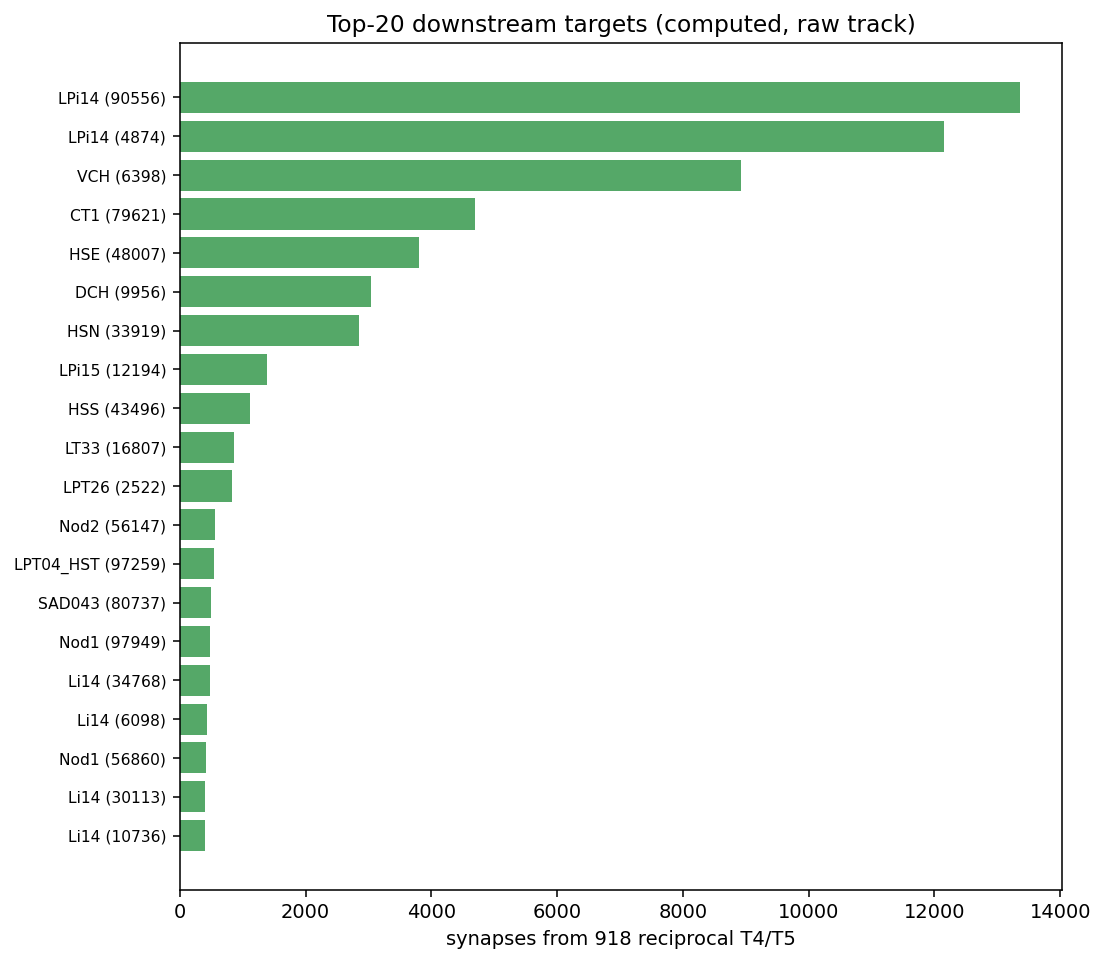
\includegraphics[width=0.80\textwidth]{downstream_top20.png}
\caption{Top twenty individual downstream targets of the reciprocal T4/T5, computed from
the raw v783 table. The identified, proofread targets (LPi14, CT1, HS cells, VCH itself,
Nodulus neurons) match the report's ranking; they are the visible tip above the 102{,}118
unannotated fragments that dominate the raw target count.}
\label{fig:top20}
\end{figure}

\begin{figure}[H]
\centering
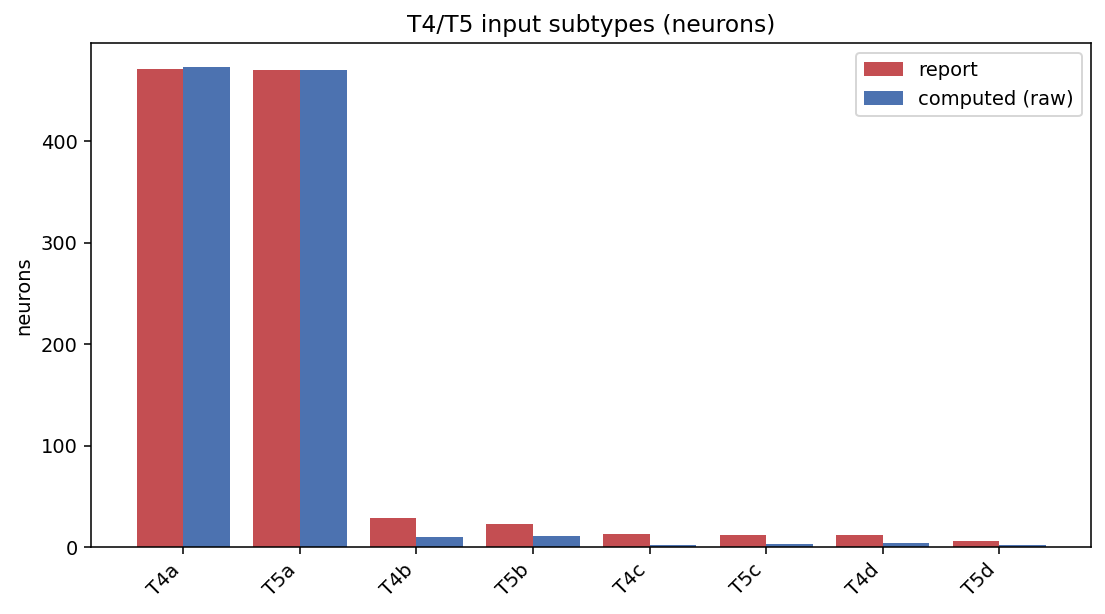
\includegraphics[width=0.80\textwidth]{subtypes_in.png}
\caption{T4/T5 input neurons by subtype, report versus computed. The dominant T4a and T5a
populations are reproduced almost exactly; only the absolute synapse mass shifts with
proofreading, leaving the subtype structure intact.}
\label{fig:subtypes}
\end{figure}

\section{Conclusions and Recommendations}

\key{The VCH and T4/T5 report is qualitatively sound but quantitatively inflated by
provenance.} Every absolute count it reports is higher than the frozen v783 dump can
justify, and the discrepancy decomposes cleanly into two proofreading mechanisms: edits
applied to the live service after the snapshot was frozen, and the inclusion of
non-proofread fragments as partners.

\key{The single most consequential takeaway is that partner counts are meaningless
without a stated proofreading policy.} The downstream-target figure swings by an order of
magnitude depending on whether non-proofread fragments are counted, and 90 percent of the
report's headline target population turns out to be unrefined fragments rather than
identified neurons.

For future reports we recommend three practices. \key{State the materialization snapshot
and the exact query date}, since the live service drifts from any fixed version. \key{Report
proofread-only and all-partner counts side by side}, so readers can see the fragment mass
explicitly. \key{Define ``annotated'' and ``tagged'' operationally} before making
completeness claims, since the proofread-versus-unproofread axis dominates any
hemispheric one.

The full machine-readable per-claim verdicts are in
\texttt{verification\_results.json}, and the complete pipeline is reproducible via
\texttt{scripts/vch\_extract.py} and \texttt{scripts/vch\_verify.py}.

\end{document}
